% !TEX root = ../presentation.tex
% !BIB program = biber
% !TEX program = xelatex

\section[Hierarchical VAEs Know What They Don't Know]{hierarchical vaes know what they don't know}


\frame{
    \frametitle{Defining OOD detection}
    \begin{columns}
        \begin{column}{0.5\textwidth}
            Enable models to distinguish the training data distribution $p(\xb)$ from any other distribution $\tilde{p}(\xb)$.
            \vspace{3mm}

            Do this for any given single observation, i.e. answer the question:
            
            \vspace{3mm}
            \begin{center}
                "Was $\xb$ sampled from $p(\xb)$ or not?"
            \end{center}
        \end{column}
        \begin{column}{0.5\textwidth}
            \begin{figure}[\textwidth]
                \centering
                \begin{tikzpicture}
                        \begin{axis}[
                            name=axistop,
                            domain=0:13,samples=100,
                            height=4.5cm, width=8cm,
                            xtick=\empty,
                            every axis plot/.append style={very thick,smooth}
                        ]
                            \addplot [name path=p1, color=red!50!black] {gauss(5,1)};
                            \addplot [name path=p2, color=black] {gauss(8,1)};
                            \path[name path=axis] (axis cs:0,0) -- (axis cs:10,0);
                            \addlegendentry{$p(\xb)$}
                            \addlegendentry{$\tilde{p}(\xb)$}
                        \end{axis}
                        \path (axistop.south) ++ (0,-0.4cm) coordinate (test);
                        \begin{axis}[
                            name=axisbottom,
                            anchor=north,
                            shift=(test),
                            domain=0:13,samples=100,
                            height=4.5cm, width=8cm,
                            every axis plot/.append style={very thick,smooth}
                        ]
                            \addplot [name path=p1, color=red!50!black] {gauss(4,0.5)};
                            \addplot [name path=p2, color=black] {gauss(9,0.5)};
                            \path[name path=axis] (axis cs:0,0) -- (axis cs:10,0);
                            \addlegendentry{$p(\xb)$}
                            \addlegendentry{$\tilde{p}(\xb)$}
                        \end{axis}
                \end{tikzpicture}
            \end{figure}
        \end{column}
    \end{columns}

    \note[item]{Define OOD}
    \note[item]{In 1D it is easy to see when this is possible and when it is not.}
    \note[item]{In higher dimensions it is not as easy to see.}
}


\frame{
    \frametitle{In distribution?}
    \begin{figure}[\textwidth]
        \centering
        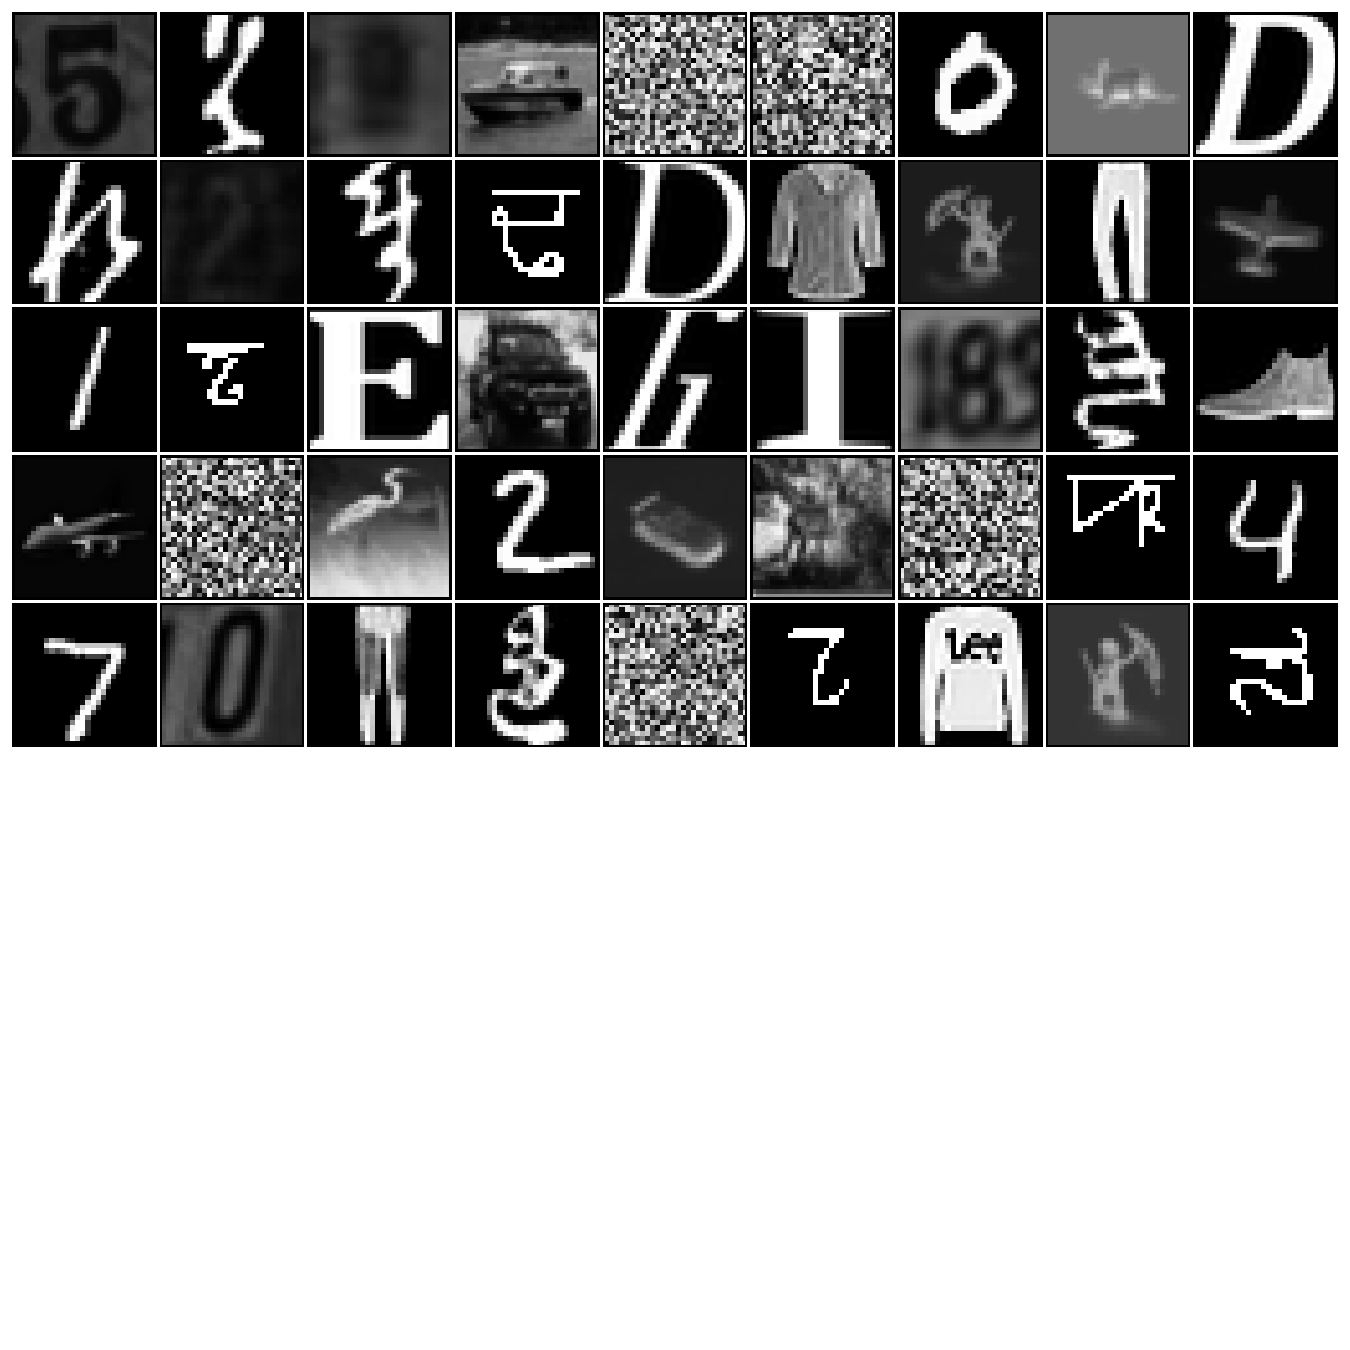
\includegraphics[scale=0.6]{figures/dataexamples_shuffled.pdf}
    \end{figure}

    \note[item]{Datasets can overlap quite a bit in their raw data space.}
    \note[item]{What we usually care about is a more semantic notion of similarity.}
}


\frame{
    \frametitle{Out of distribution?}
    \begin{figure}[\textwidth]
        \centering
        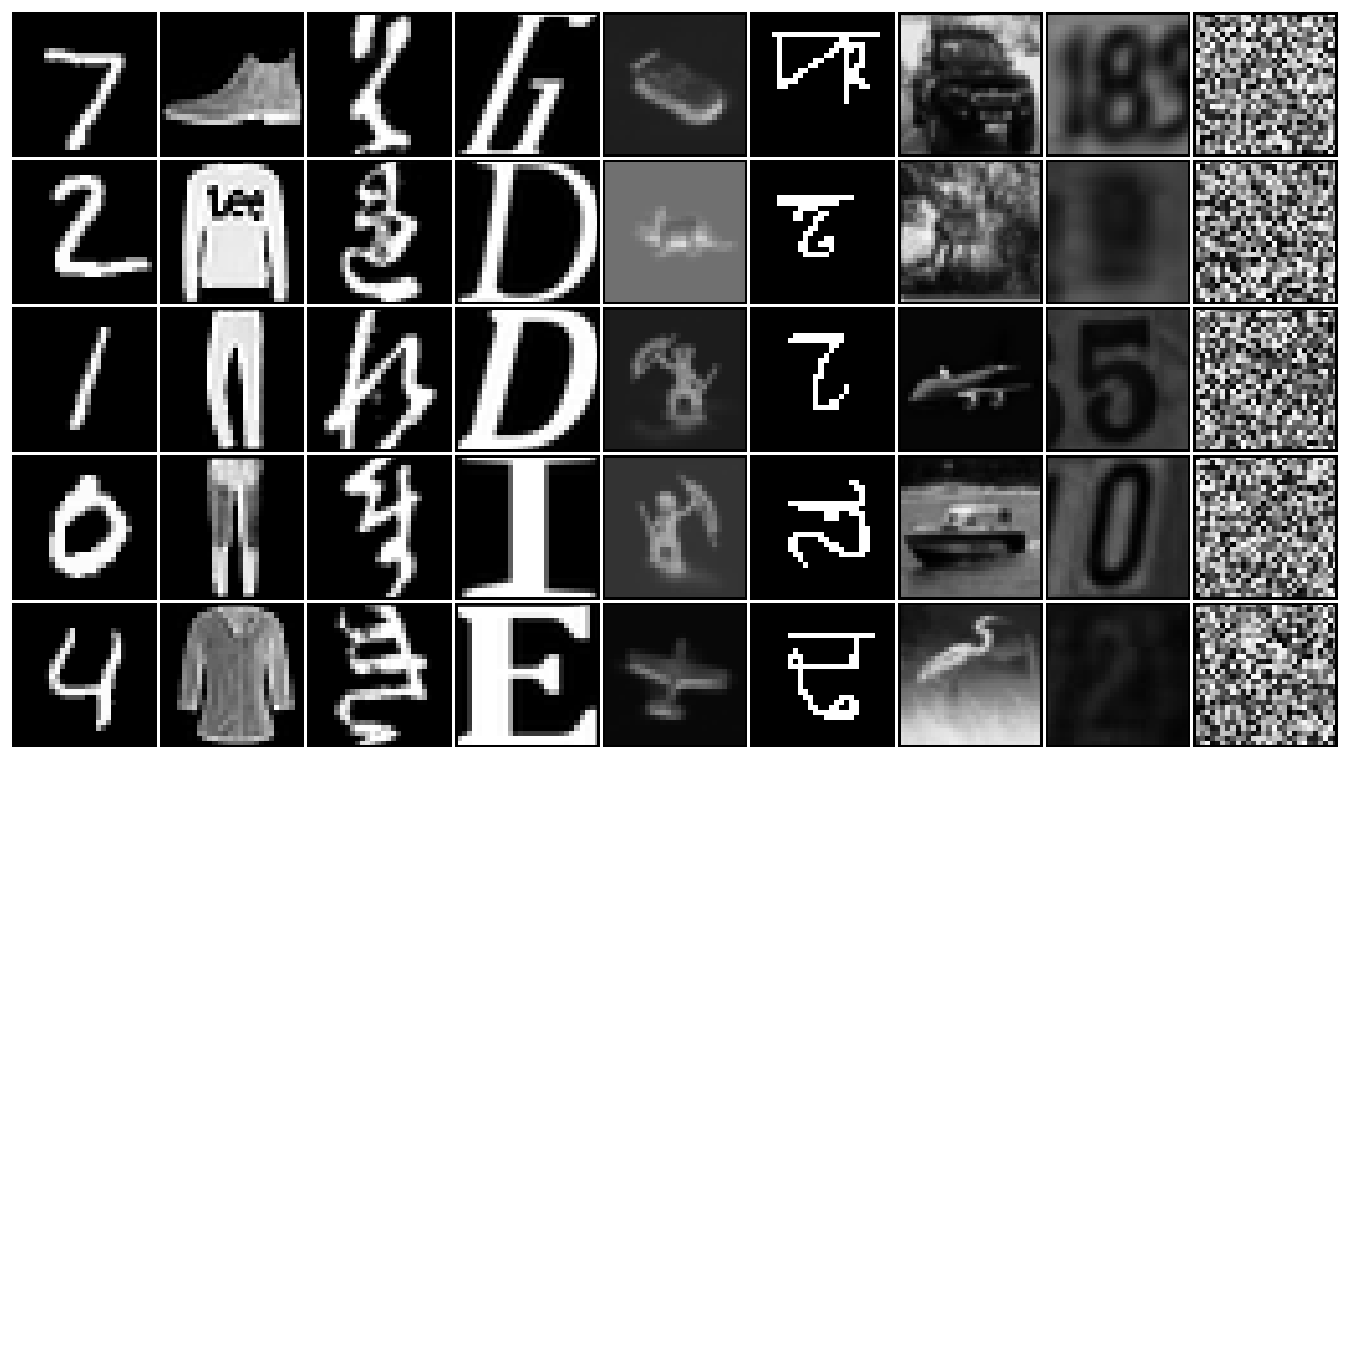
\includegraphics[scale=0.6]{figures/dataexamples.pdf}
    \end{figure}

    \note[item]{Datasets can overlap quite a bit in their raw data space.}
    \note[item]{What we usually care about is a more semantic notion of similarity.}
}


\begin{frame}
    \frametitle{Out-of-distribution detection with generative models}
    \begin{columns}[t]
        \begin{column}{0.4\textwidth}
            \begin{itemize}
                \item Generative models learn to approximate the \textbf{data distribution} $p(\xb)$.
                \item The likelihood of the model given a sample $\xb$ is a measure of how well the model \textbf{explains the data}.
                \item \textbf{Model likelihood} has long been thought of as useful for OOD detection \cite{bishop_novelty_1994}.
            \end{itemize}
        \end{column}
        \begin{column}{0.6\textwidth}
            \begin{overprint}
                \onslide<2>
                {\footnotesize HVAE trained on FashionMNIST evaluated on FashionMNIST and MNIST.}
                \begin{figure}
                    \centering
                    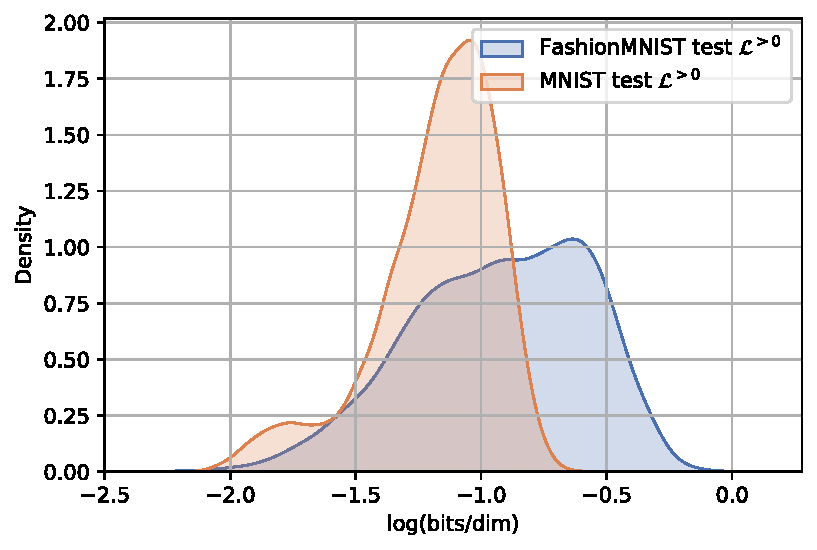
\includegraphics[width=0.8\textwidth]{../graphics/paper_hierarchical/densities-FashionMNIST-test-MNIST-test-bpp-k-0_sohau.pdf}
                \end{figure}
            \end{overprint}
        \end{column}
    \end{columns}
\end{frame}



% \frame{
%     \frametitle{Problem and Contributions}
%     \begin{itemize}
%         \item Deep generative models often fail at OOD detection task when using their likelihood estimate as the score function \cite{nalisnick_deep_2019} by, perhaps surprisingly, assigning \highlight{higher likelihoods to OOD data}.
%         \item Contributions:
%         \begin{itemize}
%             \item We provide evidence that out-of-distribution detection fails due to learned low-level features that generalize across datasets.
%             \item We present a new score for OOD detection with hierarchical VAEs that alleviates this issue.
%         \end{itemize}  
%     \end{itemize}
% }


% \section{Latent variable models}

\begin{frame}{Hierarchical VAE}
  \begin{columns}
      \begin{column}{0.7\textwidth}
          We choose the hierarchical VAE as our model \cite{kingma_autoencoding_2014, rezende_stochastic_2014}.
          \begin{equation*}
              p_\theta(\xb) = \int p_\theta(\xb,\zb) \text{d}\zb = \int p_\theta(\xb|\zb)p_\theta(\zb) \text{d}\zb
          \end{equation*}
          Specifically we use
          
          \begin{enumerate}
              \item a three-layered hierarchical VAE with bottom-up inference and deterministic skip-connections for both inference and generation.
              \begin{align*}
                  \text{Generative model: }\quad p_\theta(\xb|\zb) &= p_\theta(\xb|\zb_1) p_\theta(\zb_1|\zb_2) p(\zb_3),\\
                  \text{Inference model: }\quad q_\phi(\zb|\xb) &= q_\phi(\zb_1|\xb)q_\phi(\zb_2|\zb_1)q_\phi(\zb_3|\zb_2).
              \end{align*}
              \item a ten-layered layered Bidirectional-Inference Variational Autoencoder (BIVA) \cite{maaloe_biva_2019}.
          \end{enumerate} 
      \end{column}
      \begin{column}{0.3\textwidth}
          \begin{figure}[.5\textwidth]
          \tikz{
          % inference
          % nodes
          \node[obs] (x_inf) {$\xb$};%
          \node[latent,above=.75cm of x_inf](z1_inf){$\zb_1$}; %
          \node[latent,above=.75cm of z1_inf](z2_inf){$\zb_2$}; %
          \node[latent,above=.75cm of z2_inf](z3_inf){$\zb_3$}; %
          \node[above=of z3_inf, yshift=-1.cm] (phi) {$q_\phi(\zb|\xb)$}; 
          
          % edges
          \edge[]{x_inf}{z1_inf};
          \edge[]{z1_inf}{z2_inf};
          \edge[]{z2_inf}{z3_inf};
          \edge[dashed, bend left]{x_inf}{z2_inf};
          \edge[dashed, bend left]{x_inf}{z3_inf};
          
          % generative
          % nodes$
          \node[obs,right=0.75cm of x_inf] (x_gen) {$\xb$};%
          \node[latent,above=.75cm of x_gen](z1_gen){$\zb_1$}; %
          \node[latent,above=.75cm of z1_gen](z2_gen){$\zb_2$}; %
          \node[latent,above=.75cm of z2_gen](z3_gen){$\zb_3$}; %
          \node[above=of z3_gen, yshift=-1.cm] (theta) {$p_\theta(\xb,\zb)$}; 
          
          % edges
          \edge[]{z3_gen}{z2_gen};
          \edge[]{z2_gen}{z1_gen};
          \edge[]{z1_gen}{x_gen};
          \edge[dashed, bend left]{z2_gen}{x_gen};
          \edge[dashed, bend left]{z3_gen}{x_gen};
          }
          \end{figure}
      \end{column}
  \end{columns}
\end{frame}

% \section{Identifying the issue}


\frame{
    \frametitle{What is wrong with the ELBO for OOD detection?}
    We can split the ELBO into two terms
    \begin{equation}
        \mathcal{L}(\xb;\theta,\phi) 
        = \mathbb{E}_{q_\phi(\zb|\xb)} \left[ \log \frac{p_\theta(\xb,\zb)}{q_\phi(\zb|\xb)} \right] 
        = \underbrace{\mathbb{E}_{q_\phi(\zb|\xb)}[\log p_\theta(\xb|\zb)]}_{\text{reconstruction likelihood}} - \underbrace{D_{\mathrm{KL}}( q_\phi(\zb|\xb) \parallel p(\zb))}_{\text{regularization penalty}} \ .
    \end{equation}
    The first term is high if the data is well-explained by $\zb$.
    The second term we can rewrite as,
    \begin{equation}
        D_{\mathrm{KL}}( q_\phi(\zb|\xb) \parallel p(\zb)) = \mathbb{E}_{q_\phi(\zb|\xb)} \Big[ \textstyle\sum_{i=1}^{L-1} \log \frac{p_\theta(\zb_i|\zb_{i+1})}{q_\phi(\zb_i|\zb_{i-1})} + \log \frac{p_\theta(\zb_L)}{q_\phi(\zb_L|\zb_{L-1})} \Big] \ .
    \end{equation}
    Since the individual terms are computed by summing over the dimensionality of $\zb_i$, the absolute log-ratios grow with $\mathrm{dim}(\zb_i)$.

    Since the lower-most latent variables are usually higher dimensional than top ones, these are weighted higher in the ELBO.

    \vspace{3mm}

    \note[item]{There is a tendency for the lower-most latent variables to be weighted higher than the higher ones.}
}


\frame{
    \frametitle{What do the lowest latent variables code for?}
    
    Absolute Pearson correlations between data representations in all layers of the inference network of a hierarchical VAE trained on FashionMNIST and of another trained on MNIST. 
    \vspace{0.3cm}

    Correlation computed between the representations of the two different models given the same data, FashionMNIST (top) and MNIST (bottom).
    
    \begin{figure}[\textwidth]
        \centering
        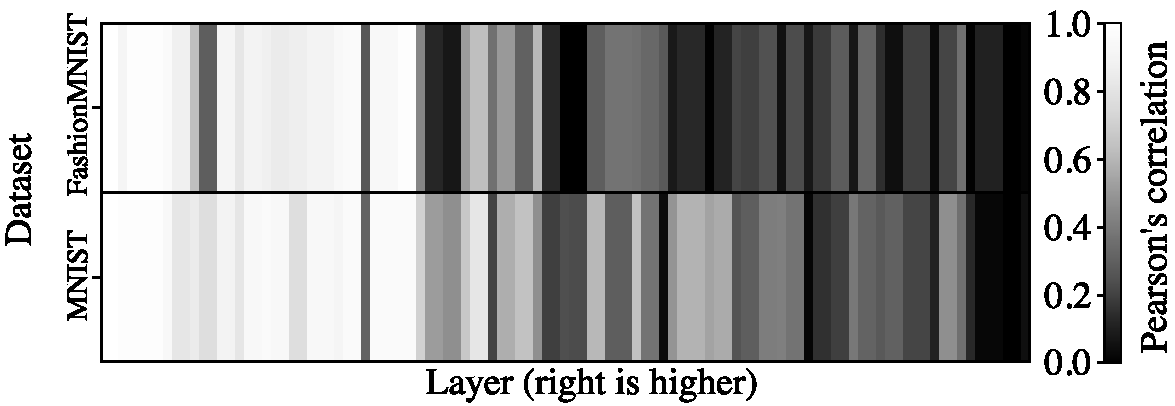
\includegraphics[scale=0.75]{../graphics/paper_hierarchical/feature-correlation-heatmap2.pdf}
        % \caption{Caption}
        % \label{fig:my_label}
    \end{figure}

    \note[item]{Strong evidence that the lowest latent variables are generalizing across datasets.}
}


% \section{The $\mathcal{L}^{>k}$ likelihood bound}


\frame{
    \frametitle{An alternative likelihood bound, $\mathcal{L}^{>k}$}
    An alternative version of the ELBO that only partially uses the approximate posterior can be written as \cite{maaloe_biva_2019}
    \begin{equation}
        \mathcal{L}^{>k}(\xb; \theta, \phi) = \mathbb{E}_{p_\theta(\zb_{\leq k}|\zb{>k})q_\phi(\zb_{>k}|\xb)} \left[ \log \frac{p_\theta(\xb|\zb)p_\theta(\zb_{>k})}{q_\phi(\zb_{>k}|\xb)} \right]
    \end{equation}
    
    Here, we have replaced the approximate posterior $q_\phi(\zb|\xb)$ with a different proposal distribution that combines part of the approximate posterior with the conditional prior, namely
    
    $$p_\theta(\zb_{\leq k}|\zb_{>k})q_\phi(\zb_{>k}|\xb)$$
    
    This bound uses the conditional prior for the lowest latent variables in the hierarchy.

    \note[item]{So can we come up with a new bound that does not use the lowest latent variables in the same way?}
    \note[item]{So we could use this for OOD detection (as done in BIVA).}
}


% \section{Likelihood ratio}


\frame{
    \frametitle{Likelihood ratios}
    We can use our new bound to compute the score used in a standard likelihood ratio test \cite{buse_likelihood_1982}.
    \begin{equation}\label{eq:llr-as-difference-in-likelihoods}
        LLR^{>k}(\xb) \equiv \mathcal{L}(\xb) - \mathcal{L}^{>k}(\xb) \ .
    \end{equation}
    We can inspect what this likelihood-ratio measures by considering the exact form of our bounds.
    \begin{align}
        \mathcal{L}      &= \log p_\theta(\xb) - D_{\mathrm{KL}}\left( q_\phi(\zb|\xb) \parallel p_\theta(\zb|\xb)\right), \label{eq:likelihoods-as-exact} \\ 
        \mathcal{L}^{>k} &= \log p_\theta(\xb) - D_{\mathrm{KL}}\left( p_\theta(\zb_{\leq }|\zb_{>k}) q_\phi(\zb_{>k}|\xb) \parallel p_\theta(\zb|\xb)\right) \notag \ .
    \end{align}
    In the likelihood ratio the reconstruction terms cancel out and only the KL-divergences from the approximate to the true posterior remain.
    \begin{align}\label{eq:llr-as-kls}
        LLR^{>k}(\xb) &= - D_{\mathrm{KL}}\left( q_\phi(\zb|\xb) \parallel p_\theta(\zb|\xb)\right) \\
                     &\quad + D_{\mathrm{KL}}\left( p_\theta(\zb_{\leq }|\zb_{>k}) q_\phi(\zb_{>k}|\xb) \parallel p_\theta(\zb|\xb)\right) \ . \notag
    \end{align}

    \note[item]{Write likelihood-ratio using the exact form of the bounds including intractable KL-divergence.}
}


\frame{
    \frametitle{Importance sampling the ELBO}
    The importance weighted autoencoder (IWAE) bound is tight with the true likelihood in the limit of infinite samples, $S\rightarrow\infty$ \cite{burda_importance_2016},
    \begin{equation}\label{eq:iw-bound}
        \mathcal{L}_{S} = \mathbb{E}_{q(\zb|\xb)}\left[ \log \frac{1}{N} \sum_{s=1}^{S} \frac{p(\xb, \zb^{(s)})}{q(\zb^{(s)}|\xb)} \right] \leq \log p_\theta(\xb) \ ,
    \end{equation}

    \vspace{3mm}

    Consequently, by importance sampling the ELBO, $D_{\mathrm{KL}}\left( q_\phi(\zb|\xb) \parallel p_\theta(\zb|\xb)\right) \rightarrow 0$ and our likelihood ratio reduces to the KL-divergence of $\mathcal{L}^{>k}$.

    \begin{equation}\label{eq:llr-as-kls-iwae-reduced}
        LLR^{>k}_{S}(\xb) \rightarrow D_{\mathrm{KL}}( p(\zb_{\leq }|\zb_{>k}) q(\zb_{>k}|\xb) \parallel p(\zb|\xb)) \ .
    \end{equation}

    $LLR^{>k}_{S}(\xb)$ performs KL-divergence-based OOD detection using top-most latent variables.

    \note[item]{We can use the IWAE bound force the KL-divergence of the original ELBO towards zero.}
    \note[item]{Then, the likelihood ratio reduces to the KL-divergence of $\mathcal{L}^{>k}$.}
    \note[item]{We can hope that using the conditional prior for the lowest latent variables will make the KL-divergence more sensitive to OOD data in the top-most latent variables.}
}


\frame{
    \frametitle{ROC curves with $\mathcal{L}^{>k}$ and $LLR^{>k}$}
    \begin{figure}[\textwidth]
    \centering
    \begin{subfigure}[c]{0.49\textwidth}
        \centering
        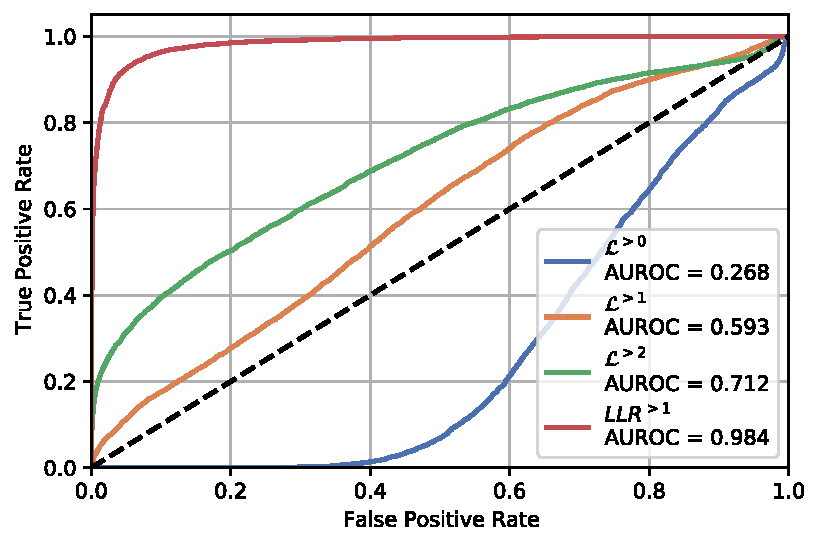
\includegraphics[width=\textwidth]{../graphics/paper_hierarchical/roc-FashionMNIST-test-MNIST-test-ll-and-llr-IW250_sohau.pdf}
        \caption{FashionMNIST HVAE evaluated on MNIST}
    \end{subfigure}
    \hfill
    \begin{subfigure}[c]{0.49\textwidth}
        \centering
        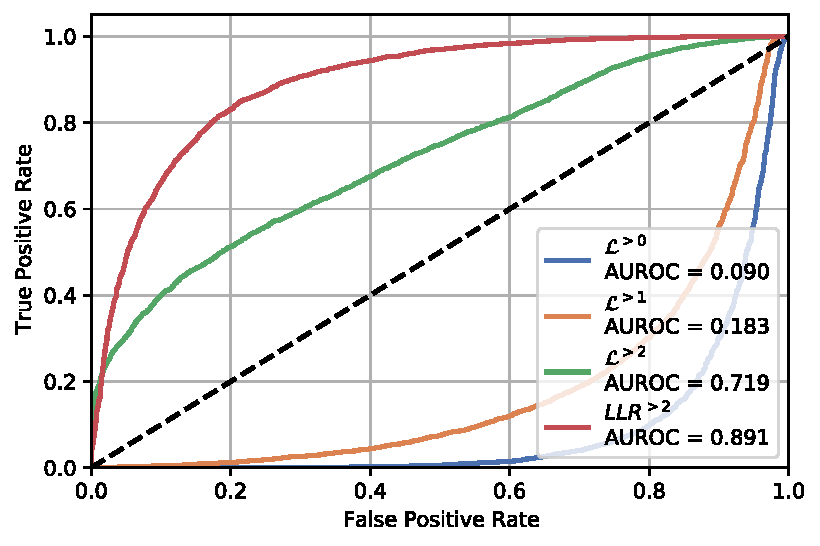
\includegraphics[width=\textwidth]{../graphics/paper_hierarchical/roc-biva-CIFAR10-SVHN-ll-and-llr_sohau.pdf}
        \caption{CIFAR10 BIVA evaluated on SVHN}
    \end{subfigure}
    \end{figure}
}


% \begin{frame}
%     \frametitle{Selecting the value of $k$}
%     \begin{itemize}
%         \item Use validation OOD dataset(s).
%         \item Compute $LLR^{>k}$ for different values of $k$ and select the one that maximizes the AUROC.
%         \item Compute feature correlations for different values of $k$ and select $k$ at the drop.
%     \end{itemize}
%     \begin{figure}
%         \centering
%         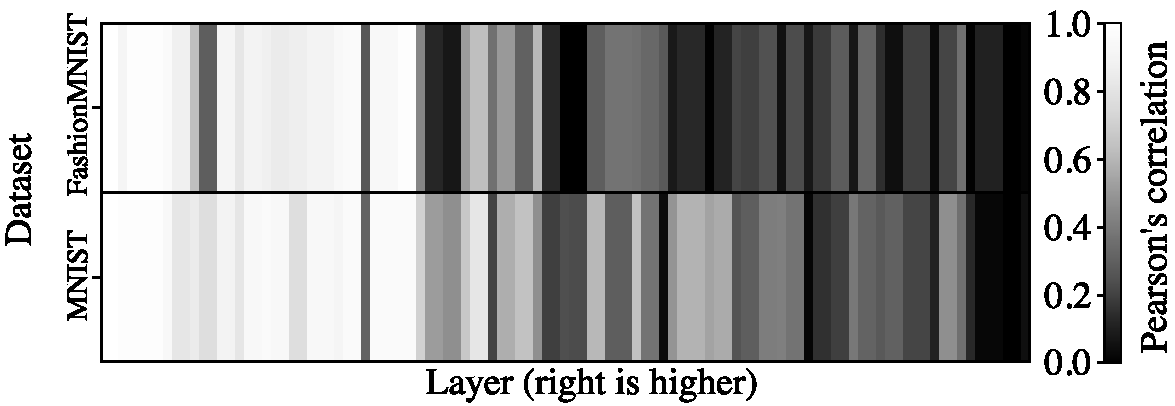
\includegraphics[width=0.9\textwidth]{../graphics/paper_hierarchical/feature-correlation-heatmap2.pdf}
%     \end{figure}
% \end{frame}


% \begin{frame}
%     \frametitle{Results on FashionMNIST/MNIST}
%     \begin{table}
%         \centering
%         \resizebox*{!}{0.87\textheight}{%
%         \begin{tabular}{lrrr}
%             \toprule
%             Method & AUROC$\uparrow$ & AUPRC$\uparrow$ & FPR80$\downarrow$ \\
%             \midrule
%             \multicolumn{4}{c}{\textbf{FashionMNIST (in) / MNIST (out)}} \\
%             \midrule
%             \multicolumn{4}{l}{\textbf{Use prior knowledge of OOD}} \\
%             Backgr. contrast. LR (PixelCNN) {\parencite{ren_likelihood_2019}}               & $0.994$ & $0.993$ & $0.001$ \\
%             Backgr. contrast. LR (VAE) {\parencite{choi_waic_2019}}                    & $0.924$ & - & - \\
%             Binary classifier {\parencite{ren_likelihood_2019}}                              & $0.455$ & $0.505$ & $0.886$ \\ % 6
%             $p(\hat{y} | \xb)$ with OOD as noise class {\parencite{ren_likelihood_2019}}     & $0.877$ & $0.871$ & $0.195$ \\ % 7
%             $p(\hat{y} | \xb)$ with calibration on OOD {\parencite{ren_likelihood_2019}}     & $0.904$ & $0.895$ & $0.139$ \\ % 8
%             Input complexity ($S$, Glow) \parencite{hendrycks_deep_2019}                    & $0.998$ & - & - \\
%             Input complexity ($S$, PixelCNN++) \parencite{hendrycks_deep_2019}              & $0.967$ & - & - \\
%             \multicolumn{4}{l}{\textbf{Use in-distribution data labels $y$}} \\
%             $p(\hat{y} | \xb)$ {\parencite{ren_likelihood_2019, hendrycks_baseline_2017}}                        & $0.734$ & $0.702$ & $0.506$ \\
%             Entropy of $p(y | \xb)$ {\parencite{ren_likelihood_2019}}                        & $0.746$ & $0.726$ & $0.448$ \\
%             ODIN {\parencite{ren_likelihood_2019, liang_enhancing_2018}}                                       & $0.752$ & $0.763$ & $0.432$ \\
%             VIB \parencite{alemi_uncertainty_2018, choi_waic_2019}                                          & $0.941$ & - & - \\
%             Mahalanobis distance, CNN {\parencite{ren_likelihood_2019}}                     & $0.942$ & $0.928$ & $0.088$ \\
%             Mahalanobis distance, DenseNet {\parencite{lee_simple_2018}}                & $0.986$ & - & - \\
%             Ensemble, 20 classifiers {\parencite{ren_likelihood_2019, lakshminarayanan_simple_2017}}                  & $0.857$ & $0.849$ & $0.240$ \\
%             \multicolumn{4}{l}{\textbf{No OOD-specific assumptions}} \\
%             \multicolumn{4}{l}{\textit{- Ensembles}} \\
%             WAIC, 5 models, VAE {\parencite{choi_waic_2019}}                          & $0.766$ & - & - \\
%             WAIC, 5 models, PixelCNN {\parencite{ren_likelihood_2019}}                      & $0.221$ & $0.401$ & $0.911$ \\
%             \multicolumn{4}{l}{\textit{- Not ensembles}} \\
%             Likelihood regret \parencite{xiao_likelihood_2020}                               & $\mathbf{0.988}$ & - & - \\
%             $\mathcal{L}^{>0}$ + HVAE (ours)                    & $0.268$ & $0.363$ & $0.882$ \\
%             $\mathcal{L}^{>1}$ + HVAE (ours)                    & $0.593$ & $0.591$ & $0.658$ \\
%             $\mathcal{L}^{>2}$ + HVAE (ours)                    & $0.712$ & $0.750$ & $0.548$ \\
%             $LLR^{>1}$ + HVAE (ours)                            & $0.964$ & $0.961$ & $0.036$ \\
%             $LLR^{>1}_{250}$ + HVAE (ours)                      & $0.984$ & $\mathbf{0.984}$ & $\mathbf{0.013}$ \\
%              \bottomrule
%         \end{tabular}%
%         }
%     \end{table}
% \end{frame}


\begin{frame}
    \frametitle{Results on CIFAR10/SVHN}
    \begin{table}
        \centering
        \resizebox*{!}{0.87\textheight}{%
        \begin{tabular}{lrrr}
            \toprule
            Method & AUROC$\uparrow$ & AUPRC$\uparrow$ & FPR80$\downarrow$ \\
            \midrule
            \multicolumn{4}{c}{\textbf{CIFAR10 (in) / SVHN (out)}} \\
            \midrule
            \multicolumn{4}{l}{\textbf{Use prior knowledge of OOD}} \\
            Backgr. contrast. LR (PixelCNN) {\parencite{ren_likelihood_2019}}               & $0.930$ & $0.881$ & $0.066$ \\
            Backgr. contrast. LR (VAE) {\parencite{xiao_likelihood_2020}}                    & $0.265$ & - & - \\
            Outlier exposure {\parencite{hendrycks_deep_2019}}                              & $0.984$ & - & - \\
            Input complexity ($S$, Glow) \parencite{serra_input_2020}                   & $0.950$ & - & - \\
            Input complexity ($S$, PixelCNN++) \parencite{serra_input_2020}             & $0.929$ & - & - \\
            Input complexity ($S$, HVAE) (Ours) \parencite{serra_input_2020} & $0.833$ & $0.855$ & $0.344$ \\
            \multicolumn{4}{l}{\textbf{Use in-distribution data labels $y$}} \\
            Mahalanobis distance {\parencite{lee_simple_2018}}                          & $0.991$ & - & -  \\
            \multicolumn{4}{l}{\textbf{No OOD-specific assumptions}} \\
            \multicolumn{4}{l}{\textit{- Ensembles}} \\
            WAIC, 5 models, Glow {\parencite{choi_waic_2019}}                          & $1.000$ & - & - \\
            WAIC, 5 models, PixelCNN {\parencite{ren_likelihood_2019}}                      & $0.628$ & $0.616$ & $0.657$ \\
            \multicolumn{4}{l}{\textit{- Not ensembles}} \\
            Likelihood regret \parencite{xiao_likelihood_2020}                               & $0.875$ & - & - \\
            $LLR^{>2}$ + HVAE (ours)                            & $0.811$ & $0.837$ & $0.394$ \\
            $LLR^{>2}$ + BIVA (ours)                            & $\mathbf{0.891}$ & $\mathbf{0.875}$ & $\mathbf{0.172}$ \\
            \bottomrule
        \end{tabular}%
        }
    \end{table}
\end{frame}


\begin{frame}
    \frametitle{Conclusions}
    \begin{itemize}
        \item Key observations: 
        \begin{itemize}
            \item The likelihood of a generative model is not a good score for OOD detection \cite{nalisnick_deep_2019}.
            \item Strong correlations between some latent variables for different datasets.
            % \item Reconstructions of OOD data are good when using full approximate posterior.
        \end{itemize}
        \item[\highlight{$\rightarrow$}] Proposed a likelihood-ratio score, $LLR^{>k}$, that uses the conditional prior for the top-most latent variables in the hierarchy and showed its effectiveness.
        % \item[\highlight{$\rightarrow$}] Showed that $LLR^{>k}$ outperforms the standard likelihood score across many different datasets and is competetive with state-of-the-art methods.
    \end{itemize}
\end{frame}

% \frame{
%     \frametitle{Results with $LLR^{>k}$}
%     % The score has good performance across many different datasets.
    
%     \begin{columns}

%     \begin{column}{0.5\textwidth}

%         \begin{table}[t]
%             \centering
%             \resizebox{0.6\textwidth}{!}{%
%             \begin{tabular}{llr}
%                 \toprule
%                  OOD dataset & Metric & AUROC$\uparrow$ \\
%                  \midrule
%                  \multicolumn{3}{c}{\textbf{Trained on CIFAR10}} \\
%                  \midrule
%         SVHN          &  $LLR^{>2}$  &  0.811 \\
%         CIFAR10       &  $LLR^{>1}$  &  0.469 \\
%                  \midrule
%                  \multicolumn{3}{c}{\textbf{Trained on SVHN}} \\
%                  \midrule
%         CIFAR10            &  $LLR^{>1}$       &  0.939 \\
%         SVHN               &  $LLR^{>1}$       &  0.489 \\
%             \bottomrule
%             \end{tabular}
%             }
%         \end{table}
%     \end{column}
    
%     \begin{column}{0.5\textwidth}
%         \begin{table}[t]
%             \centering
%             \resizebox{0.75\textwidth}{!}{%
%             \begin{tabular}{llr}
%                 \toprule
%                  OOD dataset & Metric & AUROC$\uparrow$ \\
%                  \midrule
%                  \multicolumn{3}{c}{\textbf{Trained on FashionMNIST}} \\
%                  \midrule
%         MNIST                    & $LLR^{>1}$             &  0.986 \\
%         notMNIST                 &  $LLR^{>1}$            &  0.998 \\
%         KMNIST                   &  $LLR^{>1}$            &  0.974 \\
%         Omniglot28x28            &  $LLR^{>2}$            &  1.000 \\
%         Omniglot28x28Inverted    &  $LLR^{>1}$            &  0.954 \\
%         SmallNORB28x28           &  $LLR^{>2}$            &  0.999 \\
%         SmallNORB28x28Inverted   &  $LLR^{>2}$            &  0.941 \\
%         FashionMNIST             &  $LLR^{>1}$            &  0.488 \\
%                  \midrule
%                  \multicolumn{3}{c}{\textbf{Trained on MNIST}} \\
%                  \midrule
%         FashionMNIST                   &  $LLR^{>1}$  &  0.999 \\
%         notMNIST                       &  $LLR^{>1}$  &  1.000 \\
%         KMNIST                         &  $LLR^{>1}$  &  0.999 \\
%         Omniglot28x28                  &  $LLR^{>1}$  &  1.000 \\
%         Omniglot28x28Inverted          &  $LLR^{>1}$  &  0.944 \\
%         SmallNORB28x28                 &  $LLR^{>1}$  &  1.000 \\
%         SmallNORB28x28Inverted         &  $LLR^{>1}$  &  0.985 \\
%         MNIST                          &  $LLR^{>2}$  &  0.515 \\
%                  \bottomrule
%             \end{tabular}
%             }
%             % \caption{Additional results for the HVAE model trained on FashionMNIST. All results computed with 1000 importance samples.}
%             % \label{tab:additional-results-fashionmnist}
%         \end{table}
%     \end{column}

%    \end{columns}
%}
